
%\font\bfbig=cmbx10 scaled\magstep4  
%\font\bftitle=cmbx10 scaled\magstep1
%\font\smbftit=cmbx10 scaled\magstep2
%\font\amb=cmtt10 scaled\magstep0
%\font\bgtt=cmtt10 scaled\magstep1

% The "twoside" in documentstyle sets positioning of 
% page numbers on the page./
%   \documentstyle[fullpage,twoside]{report}
\documentclass{report}
\addtolength{\hoffset}{-15mm}
\addtolength{\textwidth}{3cm}
\addtolength{\textheight}{3.5cm}
\usepackage{makeidx,graphicx}
\makeindex

\begin{document}

\title{
\begin{figure}[!h]
\centering

\includegraphics[width=15cm]{Hawk2.png}
\label{hawk-cover}
\end{figure}
\vspace {1.0in}
{User Manual} \\ Version 1.0 (Alpha) }
\author {Filipe Maia}

\maketitle

\parindent=0pt 
\baselineskip=18pt 
\lineskip=0pt
\pagenumbering{roman}

\tableofcontents

\pagestyle{headings}

\def\delfo{$\delta_{fo}$~}
\def\delfc{$\delta_{fc}$~}
\def\qq{\qquad\qquad}
\def\hbar{\overline{h}}


% OFF WE GO .......

\chapter{Introduction} 
\label{intro}
\pagenumbering{arabic}

\vspace {0.1in}

Hawk is a collection of computer programs which aim at reconstructing an object from 
it's oversampled  diffraction pattern. This usually means diffraction patterns from 
single particle diffraction, as opposed to crystal diffraction. An oversampled diffraction
 pattern is simply a diffraction pattern which can be sampled more finely than a crystal
 of the same sample. This progrm makes use of many different algorithms which all take
 advantage of the fact that in real space an oversampled diffraction pattern causes 
the solution to be surrounded by an empty region, which can be used be used to 
constraint the possible phases for the diffraction pattern ~\cite{Miao2000}.

\chapter{Learning by Example}
\label{tutorial}


We're gonna start by trying to reconstruct a simple object, a ring. I'm going
 to assume you have Hawk installed and all the programs are in the path. If
 this is not the case please read the Installation chapter~\ref{installation}.

\section{First contact with Hawk}
\label{tutorial-ring}

For this reconstruction we're gonna start with a preprocessed diffraction pattern.
 The preprocessing involves masking out overexposed pixels, removing background and 
beamstop, and other trivialities which are nevertheless important, but which we can
 learn more about later. For the moment we'll focus on the inversion problem alone. 
To begin with you need to go to the Hawk website and download the examples package if
 you haven't done it yet. Then just decompress it and change your current directory
 to the newly created ``examples/ring'' directory.

\vspace {0.1 in}

\qq {\tt  \$ tar -zxf examples.tar.gz}


\qq {\tt  \$ cd examples/ring}

Now inside this directory there should be two files called ``ring.h5'' and ``uwrapc.conf''.
The first file has the experimental data that we are trying to reconstruct.
It contains things like image intensity at each point, a mask, image center
and other important information. For a more detailed description of the format
please check the file format reference~\ref{file-format-hdf5}. 
The second one
contains the options that are passed to the solver. This is the file that controls
the solver and is {\em always} named ``uwrapc.conf''. Here's how it looks like:

\begin{verbatim}
# File containing the diffraction pattern
  amplitudes_file = "ring.h5";
# Threshold of the autocorrelation which defines the initial guess
  patterson_threshold = 0.01000000;
# Threshold for defining the new support after each support update
  support_intensity_threshold = 0.100000000;
# Number of iterations untill the minimum blurring is reached
  iterations_to_min_blur = 4000;
# Reconstruction algorithm used
  algorithm = "RAAR";
# Use random intensities for the non zero part of the initial guess
  random_initial_intensities = 1;
# Directory where to do the reconstructions
  work_directory = ".";
# Algorithm for support update
  support_update_algorithm = "fixed";
# Make all amplitudes relative to maximum 
  rescale_amplitudes = 1;
\end{verbatim}

It's a simple key = value configuration file. All lines starting with ``\#'' are
comments and not interpreted by the program. Don't worry if you don't understand all lines.
It might be a good idea to take a look at the Basic Algorithm chapter~\ref{basic-algorithm}
if all this seems alien to you. 

Now lets run the program and see what output it produces.

\qq {\tt  \$ uwrapc}

A word of warning, the program {\em never} stops so you are responsible to kill it when you're satisfied
with the results. 

Using another shell you can take a look at the files being created in that directory.
First a file called uwrapc.confout will be created which lists all the options you chose, plus the defaults
that were used. Don't be afraid by it's length, many options are irrelevant for most reconstructions.

Another file created is diffraction.png, which contains a color coded representation of the pattern being
phased. The file autocorrelation.png shows the patterson function of your diffraction pattern and the files
``initial\_guess.png'' and ``initial\_support.png'' are obviously the first guess for the
 iterative algorithm and the
 first support, respectively. You should take a quick look at them all to see if everything is running as
 expected. 

Within some time the program start to output files named ``real\_out-xxxxxxx'' and 
``support-xxxxxxx'' where the x's represent a number. This is simply the output of the program 
after xxxxxxx iterations. The output is stored in color coded png file for quick inspection and in h5
 files for more rigorous future analysis. The remaining file created by the program is uwrapc.log and it
contains numerous statistics useful for checking the evolution of the reconstruction. You can look at 
this file using Grace, which is freely available on the internet, with the following command:

xmgrace -nxy uwrapc.log

The most interesting plots are probably the Fourier Error and Real Space Error. For more information about
 the log file check the appropriate chapter ~\ref{Log-File}.

After about 20000 iterations or so the program should have reached a stable solution, so you can kill it.
You can check the final values of the Fourier and Real Space Errors in the log file and visually inspect the
reconstructed image. Hopefully it should look something like this:

\begin{figure}[htp]
\centering
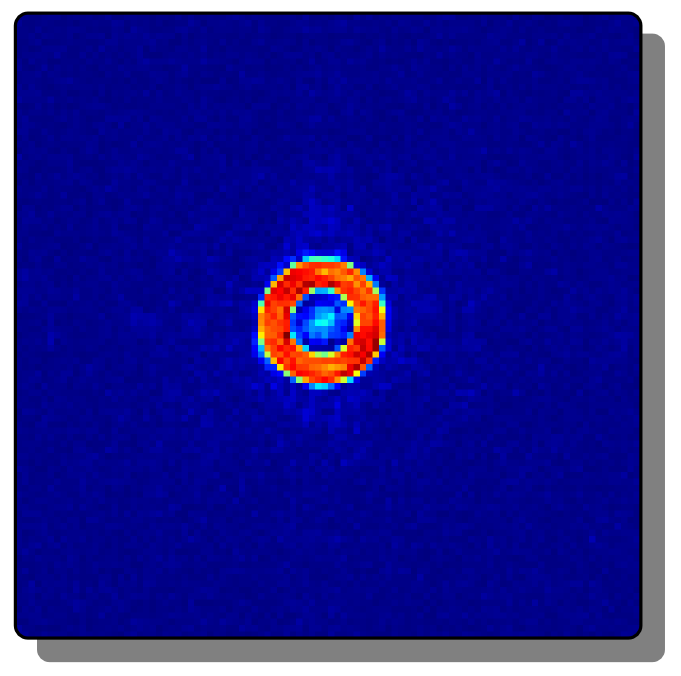
\includegraphics[scale=0.5]{reconstructed_ring.png}
\caption{Colormap representation of the reconstructed ring.}
\label{reconstructed-ring}
\end{figure}

{\bf Congratulations, you have just finished your first reconstruction!}



\section{Ring preprocessing}
\label{tutorial-ring-preprocessing}

Prepocessing is necessary because unfortunately in the real word pixels saturate, there's background noise, 
there are beamstops and other problems that make life more difficult. Prepocessing might also be desirable
to reduce image size throwing away redudant information in order to speed up calculation.
So in Hawk there's a program called
``process\_image'' which will take your raw experimental image and massage it so it becomes suitable for further 
processing. You can start by taking a look at the raw image using a small utility bundled in called ``image\_to\_png'',
and compare it to the preprocessed one.

\vspace {0.1 in}

\qq {\tt  \$ image\_to\_png ring\_raw.h5 ring\_raw.png}

\qq {\tt  \$ display -resize 600x400 ring\_raw.h5 \&}

\qq {\tt  \$ image\_to\_png ring.h5 ring.png}

\qq {\tt  \$ display -resize 400x400 ring.png \&}

\begin{figure}[htp]
\centering
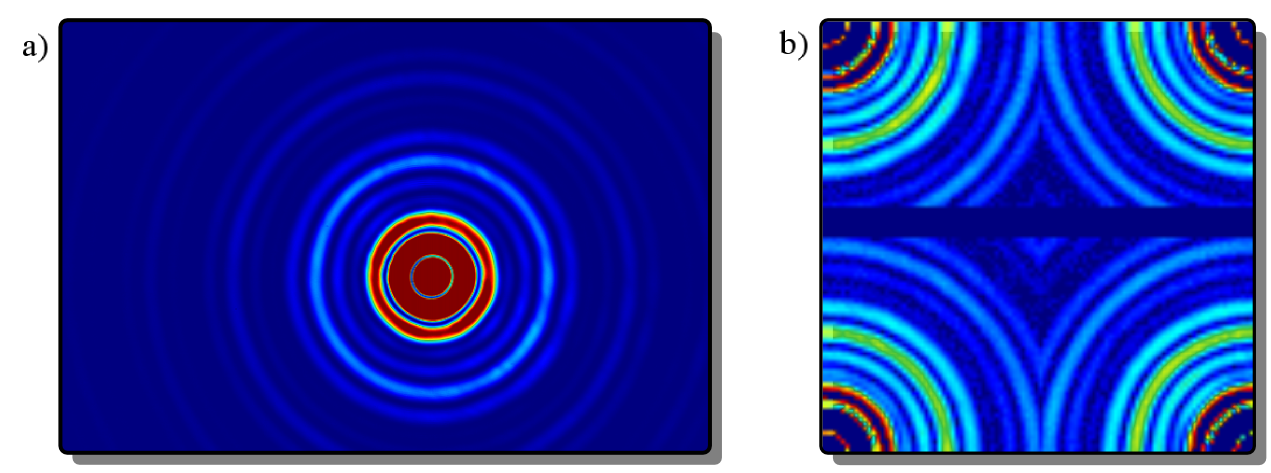
\includegraphics[scale=0.3]{ring_data_comparison.png}
\caption{a) Log scale colormap of the raw ring data. b) Log scale colormap of the processed ring data.}
\label{data-comparision}
\end{figure}

The first thing you'll probably notice is that the processed one doesn't look at all like rings, and it's also much smaller.
One of the effects of preprocessing is to swap the quadrants of the picture with respect to the center of the diffraction pattern.
To do this it will try to figure out the center of the image by using the maximum of the self convolution as the center.
Alternatively it can also be specified by the user.

\begin{figure}[htp]
\centering
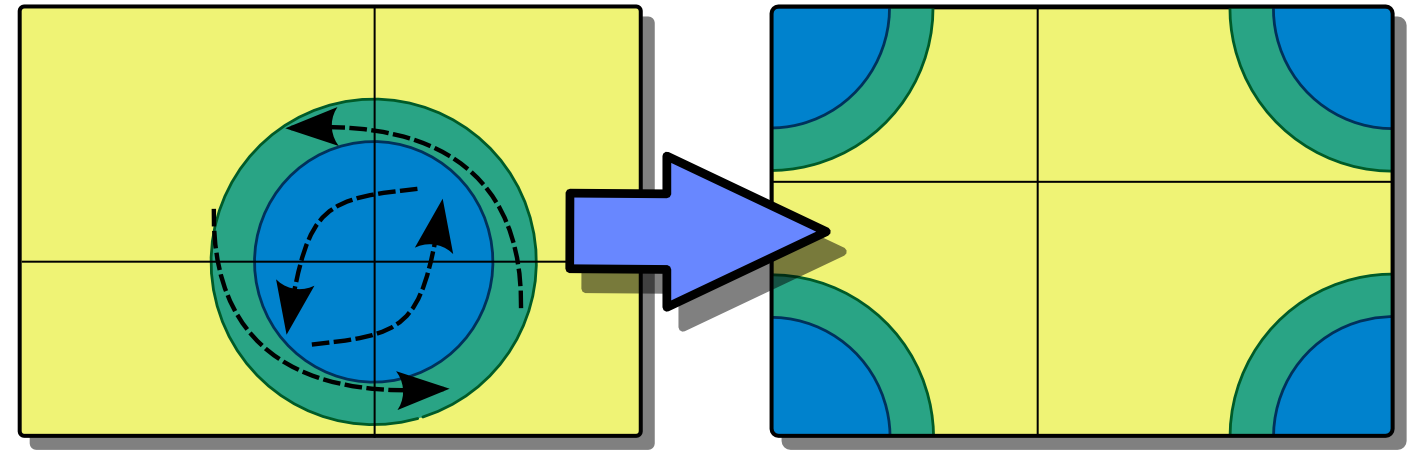
\includegraphics[scale=0.25]{fft_shift.png}
\caption{Quadrant swapping data, for compatibility with FFTW}
\label{quadrant-swapping}
\end{figure}

Another interesting difference between the two images images is that the processed one is square while the raw is rectangular.
For the moment Hawk can only image with square image so the input has to be cropped to make it square.
A last important difference is that the processed image has zeroes(blue) where the raw image has saturated pixels near the center
of the diffraction pattern. These zeroes are not really zeroes, they are just unkown values. Inside ring.h5 besides the image itself
there's also a mask that specifies which values have experimental meaning and which do not. We can take a look at it by doing (figure ~\ref{ring-mask}):

\qq {\tt  \$ image\_to\_png ring.h5 ring.png ring\_mask.png \&}

\qq {\tt  \$ display -resize 400x400 ring\_mask.png \&}

\begin{figure}[htp]
\centering
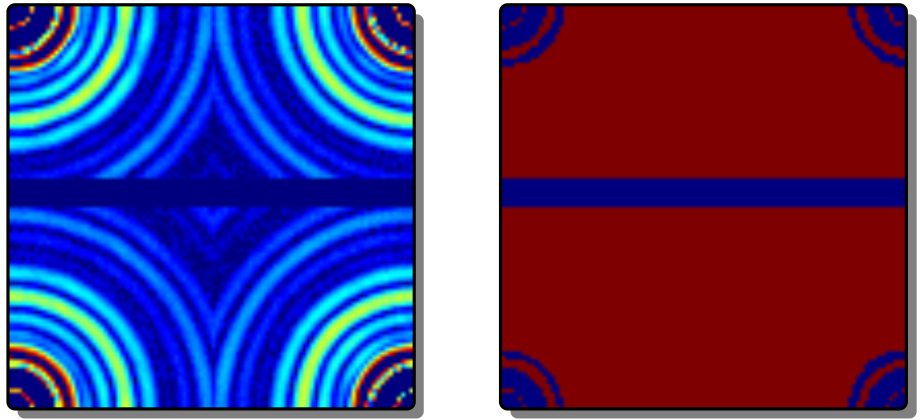
\includegraphics[scale=0.4]{ring_and_mask_svg.png}
\caption{Ring image with mask next to it. The blue represent unmeasured data, and red the opposite.}
\label{ring-mask}
\end{figure}

You can see that there are quite a few regions with zero in the mask, which correspond to experimentally unkown intensities.
The area close to the corners of the mask correspond to saturated pixel detectors (this area actually corresponds to the
center of the detector). The horizontal strip in middle of the mask is due to a completely different reason. Because
Hawk can only deal with square images, the images are first made square by padding the smallest dimension with zeroes untill
the image becomes square. Obviously the padding values don't have any real meaning so they are masked out.


Now that we know a bit more about images and masks lets try to process our image.
We'll start by examining the image to determine at which point the detector seems to saturate.
An easy way to examine images is to use an excellent visualizer called VisIt produced by the LLNL
and freely available for many platforms. Please visit the page http://www.llnl.gov/visit/ for
more information, including installation details. From now on i'll assume that you have VisIt installed.


VisIt cannot open the image format used by Hawk so we'll have to convert it to some standard format. We'll use 
image\_to\_vtk to do just that:

\qq {\tt  \$ image\_to\_vtk raw\_ring.h5 raw\_ring.vtk \&}

This will transform the image into a 2D structured points VTK file.
You can now start VisIt and load the file (File->Select File, chooses the files and hit select).
Draw the image using Pseudo color (select the file from the list box, press open, 
then go to Plots and choose pseudocolor, and you maybe need to hit the Draw button now).


You should be able to see now the raw image (figure ~\ref{visit-raw-ring}):

\begin{figure}[htp]
\centering
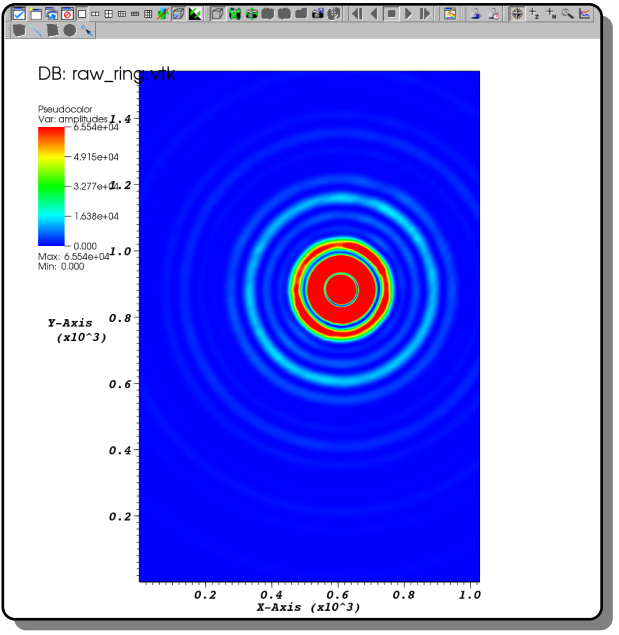
\includegraphics[scale=0.4]{visit_raw_ring.png}
\caption{Pseudocolor representation of the raw ring image.}
\label{ring-mask}
\end{figure}

You can now use use the Node picking tool to check the red values close to the center. The highest value you'll
find is 65535, but we should set the saturation limit somewhat below let, lets say 55000.
We should now try to determine more or less the background. For this it's better to change the color scale to 
logarithmic (on the Active plots list click on the arrow on the left side of the first plot, double click  on
the tree member ``Pseudocolor'', select Min and set it to 1, and then select log scale).
You can see that there seems to be plenty of signal all the way to high resolution, and the background seems
very small. So we can safely set the background to 0. 


Another important thing to notice about this diffraction pattern is that it's quite smooth. This means that it's
higly oversampled. To reduce computing time we can downsample it. We can for example first try to downsample it by
3x. So lets put all of this into a command:

\qq {\tt  \$ process\_image -i raw\_ring.h5 -o pro1\_ring.h5 -s 55000 -g 0 -a 3}

This command will transform the intensities into amplitudes, do the required fft shifts, mask out all intensities
above 55000, remove the background from our picture and downsample it by 3x.
It's always a good idea to visually inspect the output to make sure it is what you expect (you have to convert it
first with either image\_to\_png or image\_to\_vtk when quantitative analysis is required).


We can now use the configuration file provided in the examples to try to reconstruct our new file.
So create a new directory, for example ``pro1'' and copy pro1\_ring.h5 and uwrapc.conf there.
Edit uwrapc.conf to replace the amplitudes\_file value with ``pro1\_ring.h5'' instead of ``ring.h5''.
Now simply run uwrapc and check the result. You'll notice that the iterations take a lot longer than 
with the ring.h5 file provided. This is because the image we're using is much larger. One important
thing to check then is the ``autocorrelation.vtk'' file. This file unsurprisingly contains the autocorrelation
of the input. If you see a lot of blank space around the autocorrelation of the object you can usually further
downsample the diffraction pattern to improve the speed of the algorith. As long as most of the autocorrelation
fits inside the image, downsampling should not be a problem ~\cite{Miao1998}. It should be noted though that 
decreasing the oversampling ratio will increase the noise so it's use depends on the signal to noise ratio
of your particular dataset.


If you are tired of waiting for the solution you can kill the process and try out an image
with a lower oversampling ratio. Instead of downsampling 3x lets try with 10x and see what happens.

\qq {\tt  \$ process\_image -i raw\_ring.h5 -o pro2\_ring.h5 -s 55000 -g 0 -a 10}

Again create another directory copy uwrapc.conf and ro2\_ring.h5 there and do the required changes in uwrapc.conf.
Run uwrapc and check out the output.



\chapter{Reference}

\section{Algorithms}
\label{Algorithms}

The following algorithms are implemented in Hawk:

\begin{itemize}
\item \textbf{HIO} - Hybrid Input-Output. For more information check ~\cite{Fienup1978} and ~\cite{Fienup1982}


\item \textbf{RAAR} - Relaxed Averaged Alternating Reflectors. For more information check ~\cite{Luke2005}


\item \textbf{HPR} - Hybrid Projection Reflections. {\em Warning: this algorithm did not receive much testing.} For more information check ~\cite{Luke2003}. 


\item \textbf{CFLIP} - Charge Flipping. For more information check ~\cite{Oszlanyi2004} and ~\cite{Oszlanyi2005}. 


\end{itemize}


\section{Blur Reduction Methods}
\label{blur reduction methods}

The following bluring radius reduction methods are implemented in Hawk. They serve to reduce the bluring radius
from \textbf{initial\_blur\_radius} to \textbf{minimum\_blur\_radius} in \textbf{iterations\_to\_min\_blur} iterations
in a smooth way.

\begin{itemize}

\item \textbf{gaussian} - Gaussian reduction method. The blur radius follows the following formula:



\end{itemize}
\begin{itemize}
\item \textbf{HIO} - Hybrid Input-Output. For more information check ~\cite{Fienup1978} and ~\cite{Fienup1982}


\item \textbf{RAAR} - Relaxed Averaged Alternating Reflectors. For more information check ~\cite{Luke2005}


\item \textbf{HPR} - Hybrid Projection Reflections. {\em Warning: this algorithm did not receive much testing.} For more information check ~\cite{Luke2003}. 


\item \textbf{CFLIP} - Charge Flipping. For more information check ~\cite{Oszlanyi2004} and ~\cite{Oszlanyi2005}. 


\end{itemize}

\section{uwrap.conf Options}

Options can be either floating point numbers (marked as float), integers (marked as int) or quoted textual strings (marked as string).
 

\begin{itemize}
\item (float) \textbf{initial\_blur\_radius} - The standard deviation of the starting radius of the gaussian, in pixels, used for blurring
the real space image during the outerloop, that is used to define a new support. 3.0 is a typical value.


\item (float) \textbf{patterson\_threshold} - Defines the value that determines if a pixel is going to be used as initial support or not. Pixels with
a value greater than max(autocorrelation)*patterson\_threshold will be part of the support derived from the autocorrelation. 0.04 is a
typical value, although this depends strongly on the image.


\item (float) \textbf{beta} - Relaxation parameter used in several algorithms including HIO and RAAR. It can vary between 0 and 1, with 1 meaning
no relaxation. It's value is directly related with the instability and speed of the algorithms. 0.9 is a typical value.


\item (int) \textbf{innerloop\_iterations} - How many innerloop iterations to execute before executing an outer loop iteration. 20 is a typical value.


\item (float) \textbf{added\_noise} - How much noise to add to the input amplitudes. The value is the standard deviation of the gaussian noise with
mean 1 that is multiplied with the input ampltitude.

\item (float) \textbf{beamstop\_radius} - This defines a circle centered in the middle of the image, with a given radius, and all the pixels lying inside
that area will be marked as unknown.


\item (float) \textbf{support\_intensity\_threshold} - Defines the value that determines if a pixel is going to be used as support in the next iteration or not. 
Pixels with a value greater than max(blurred image)*support\_intensity\_threshold will be part of the support that is updated at every outerloop.
0.20 is a typical value, although this depends strongly on the image.


\item (int) \textbf{iterations\_to\_min\_blur} - How many innerloop iteration untill the bluring radius decreases to it's minimal value. Usually around 3000.


\item (float) \textbf{minimum\_blur\_radius} - Minimum bluring radius, in pixels. 0.7 is a usual value.


\item (bool) \textbf{enforce\_reality} - If not 0 the real space image will be forced to be real by setting it's imaginary part to 0.


\item (string) \textbf{logfile} - Name of the file where to write to log. Usually "uwrapc.log".


\item (int) \textbf{output\_period} - Number of innerloops between writing image files.


\item (int) \textbf{log\_output\_period} - Number of innerloops between writing output to the log file.


\item (string) \textbf{algorithm} - Name of the algorithm to use. Check section~\ref{Algorithms} for details.

\item (string) \textbf{blur_radius_reduction_method} - Method used to change the blur radius. Check section~\ref{blur reduction methods} for details.


\end{itemize}

\bibliographystyle{acm}
\bibliography{imaging}

\end{document}
 